\section{\label{sec:regexps}Regular expressions}
\fixme{This is a weird draft by Petch}

\subsection{Match as a regular expression}
The left part of the match (without the resulting type) is actually a
regular expression, but with tokens to be matched instead of single
characters. That does not change the concept, because just the same as
we can have a getter for the next symbol in the input stream, we have
the get next token function in the parser. We operate not with an input
stream of symbols, but with an input stream of pseudo-tokens.

Currently our regular expression syntax allows using or \verb/|/ and asterisk
\verb|*| notations. Asterisk is more binding than or, so if you want to have (a
or b) zero to n times you will have to write \verb/(a|b)*/. The supported
syntax can easily be extended.  For the time matching classes of tokens is
unsupported, however the classes can be emulated by using or constructions.
This is possible because the token count is fairly limited, unlike the
character set that can be used in regular expressions.

The given regular expression is parsed to create a non-deterministic automaton.

\subsection{NFA to DFA}
Next step is to create a DFA out of the created NFA to minimize the effort
needed to execute the given automata. Currently the subset construction
algorithm is used for the determinisation process. It is described in detail in
the "Dragon Book".

Then the determinate automata created is minimised. Minimisation algorithm is,
again, described in detail in the "Dragon Book". The algorithm creates sets of
states that cannot be distinguished by any input token sequence. Once the
algorithm fails to break the sets into smaller ones it stops the process. These
sets of states then become the new states of the minimal automaton.

It is essential to note that the existence of such minimal automaton is
provable, despite the complexity of the regular expression it describes. This
statement implies that we have a possibility to prove equality of two automata.
As the naming of the states is unimportant, we will say that two automata are
the same up to state names if one can be transformed to another be simply
renaming the states. Therefore two regular expressions match the same input if
and only if their automata are the same up to state names.

The created DFA is minimal and therefore the most effective for matching
the given expression. The DFA is represented by a list of objects where
each object contains a map of symbols and objects to which the current
symbol transfers the automaton.

The construction of the DFA does not support back-referencing, so the bracket
groups are intended only to change the priority of the operations in the
regular expressions. We abandon the back-referencing feature in favor of
maintaining a fully determinate automaton for each regular expression.
Consequently, in the matches' output, all of the tokens are returned in a
single unnested list. 

\fixme{is the paragraph below needed?}

We still consider an option to allow backtracking in case it will become
necessary.  If we perform determinisation only on the parts of the automaton
that are enclosed in braces and then combine the created automata by
consequently connecting the accepting and starting states together, we will
create an automaton that allows grouping. However this approach disallows the
combining of several matcher automata into a single one, as the procedure would
ruin the grouping.

\subsection{Several DFA to single DFA}
As we operate with the source code, we want to check all of the matches that we
have in one pass through the code. We will consider two possibilities to do
this, which are described below. For both of them we evaluate DFA adding,
matching and context inheritance algorithmic difficulty.

Context inheritance difficulty is important, as we can have several included
contexts, where the matches introduced inside the included one have a higher
priority. Imagining that we have a system of \verb/n/ automata we have two
options of doing so. The first one is that on entering a context we add the
\verb/m/ matches we come across to the main match set and remove the \verb/m/
matches upon exiting the context. The second one is that on entering a context
we create a copy of the parent context, to which we add the \verb/m/ newly
found matches and upon exiting the context throw out the entire new system of
matches.

We do not explicitly select a method of operation with joining DFA, we only
give the complexities of the proposed variants. This is because the optimal
solution selection should be based on the practical uses of the system. It is
impossible to state, without any actual examples, what will be more
time-effective during execution. Even though the second option is
time-consuming when adding and removing matches, the dramatic improvement in
execution time might come from the fact that match count is relatively small,
but the automaton execution will, at worst cases, be performed for every token
in the source text.

\subsubsection{List of DFA}
The simplest method of executing several DFA at one pass though the source code
is to store them in a list. Let us assume that there are \verb/n/ matches to be
checked. Then the automata list represents an NFA with \verb/n/ epsilon
branches from the start state, each of which leads to one of the DFA we already
created.

\begin{description}

\item[Match adding] \hfill \\

DFA adding in this case is simple, as the only action necessary is to add the
automaton to the list, so the complexity is $O(1)$.

\item[Matching] \hfill \\

In this case matching depends both on the count of automata \verb/n/ and on the
length of the matched pattern \verb/l/, as we have \verb/n/ branches of an NFA
to traverse simultaneously. So in the worst case the algorithmic difficulty of
the task will be $O(n*l)$.

\item[Context inheritance] \hfill \\

The first option of context inheritance can be executed easily, as the added
\verb/m/ matches can be removed from the system in a single block. So it's
complexity is $O(1)$. The creation and deletion of the whole match system also
has time complexity of $O(1)$.

\end{description}

\subsubsection{Combining several DFA into single DFA}

In this case we combine the automata created for each of the matches together
into a single DFA. This is done in order to reduce matching time. 

\begin{description}

\item[Match adding] \hfill \\

The algorithm combines the states of two automata one by one, and is, in fact,
an adaptation of the determinisation algorithm. Its complexity is $O(m*n)$,
where \verb/m/ is the amount of states in one automata, and \verb/n/ is the
amount of states in the second automata.

Imagine that we have two consequent matches, for both of which we have
generated an automaton. At first we create a starting state for the merged
automaton by combining the starting states of existing ones. Then we examine
the paths leading by same tokens from the combined states in the two starting
automata. We create states in the new automata from the end points of the paths
in the existing automata and add paths to them by the examined symbol. By doing
so for every new state we add all of the paths and create the combined
automaton. By prioritising the regular expressions we can unambiguously
identify the regular expression for which a specific state will be accepting.

The figures show an example of this algorithm execution.
Figure~\ref{fig:automaton_aastbast} shows the automaton for \verb/a*b*/. It has two
states, each of which is an accepting state. Figure~\ref{fig:automaton_ab}, on
the other hand, shows the automaton for regular expression \verb/ab/. It has 3
states, the last of which is an accepting state. Smaller circles in colors of
the state id's show that the state is accepting for the corresponding
automata.

\begin{figure}[h]
  \centering
    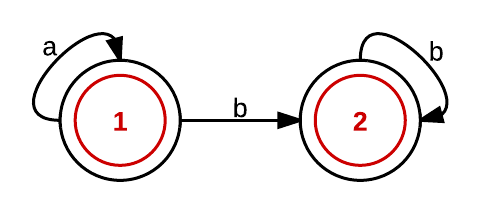
\includegraphics{automaton_2}
  \caption{Automaton for a*b*}
  \label{fig:automaton_aastbast}
\end{figure}

\begin{figure}[h]
  \centering
    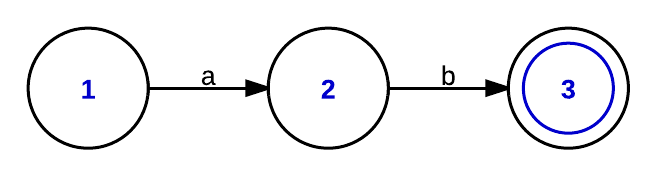
\includegraphics{automaton_1}
  \caption{Automaton for ab}
  \label{fig:automaton_ab}
\end{figure}


The algorithm traverses the two automata step by step adding new states to the
resulting one. Firstly, the state \verb/(1, 1)/ is created, which is a
combination of the two automata starting states. By symbol \verb/a/ the first
automata goes to state \verb/2/, however the second one stays at state
\verb/1/. As a result state \verb/(2, 1)/ is added together with a path to it
by token \verb/a/ from \verb/(1, 1)/. Next paths are created for the newly
added state \verb/(2, 1)/. By token \verb/b/ we add state \verb/(3, 2)/ and the
corresponding path and so on. The resulting automata is shown on
figure~\ref{fig:automata_merge}. 

\begin{figure}[h]
    \centering
    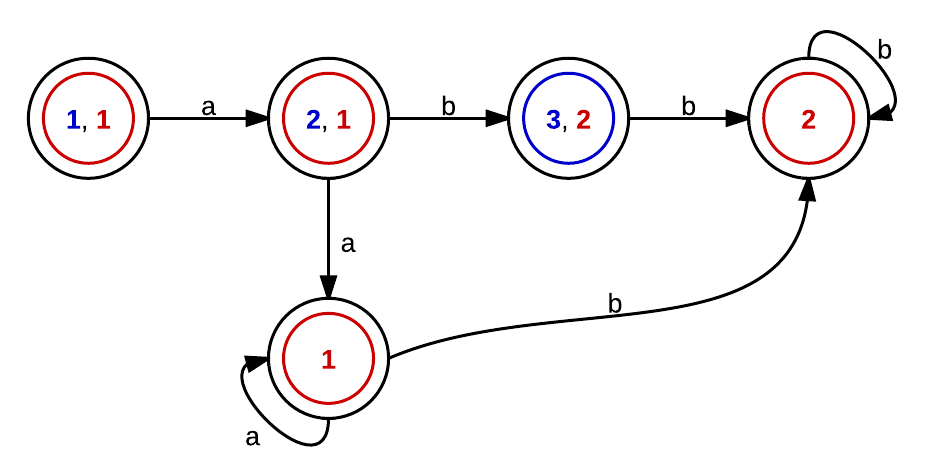
\includegraphics{automata_merge}
  \caption{Automaton for ab and a*b*}
  \label{fig:automata_merge}
\end{figure}

In figure~\ref{fig:automata_merge} the states \verb/(1, 1)/, \verb/(2, 1)/, \verb/(1)/ and \verb/(2)/ are accepting for the regular expression \verb/a*b*/, but the state \verb/(3, 2)/ is accepting for regular expression \verb/ab/. Here we assume that the first regular expression to appear has lower priority than the ones that appear later. Otherwise state \verb/(3, 2)/ would also be accepting, but for the second automata.

\item[Matching] \hfill \\

Here matching depends only on the length of the matched token list, so the
complexity is $O(l)$, as only a single automaton traverse option exists for a
single input token.

\item[Context inheritance] \hfill \\

Context inheritance by adding and removing matches is not as efficient as in
the case of automata list. Adding complexity was described above, however to
remove an amtch from the system we will have to traverse all of the automata
states and track those, that belong to the removed automata. So the complexity
of a removing of an expression, if \verb/m/ is the amount of states of the
system, will be $O(m)$.

If we adopt the second option, creation and deletion of a match system for a
nested context, the complexity will remain the same as in adding DFA to the
system, as the deletion will not add to it.

\end{description}
